\paragraph{Funcionalidades del sistema}

El usuario el sistema tendrá la capacidad de:

\begin{itemize}
    \item Un programa gestor para introducir y gestionar tareas para ejecutar en sistemas remotos de forma automática o manual.
    \item Un programa cliente para instalar en cualquier servidor con la capacidad de recibir tareas desde el manager que se ejecutarán de forma automática.
    Cualquier programa instalado en dicho servidor podrá ser ejecutado.
    \item Un programa de control instalable en cualquiera de los servidores clientes para actuar sobre un pid que controle motor de corriente continua.
\end{itemize}

\paragraph{Garantías de seguridad y calidad}\label{par:testing}
    Conforme a los principios teóricos establecidos para el diseño de tests la cobertura de este proyecto se centrará en hacer tests unitarios para el Dominio.
    En la~\cref{fig:piramidTest} se muestran las distribuciones de test que representan el ideal a la derecha y a el que tienen los sistemas a la izquierda.
    Las pruebas unitarias sólo son posibles cuando hay un buen diseño del software.
    En los proyectos que no disponen de un diseño que posibilite hacer test unitarios se ven abocados a hacer uso de tests que prueban demasiado código y características al mismo tiempo.
    Esto provoca que sean tests que tienen a fallar rápidamente y deben cambiarse habitualmente ante cualquier pequeño cambio.
    Las pruebas de más alto nivel incluyen incluso las interfaces de usuario.
    Debieran estar destinadas a funcionalidades muy establecidas y cuya tendencia al cambio sea muy escasa.

    \begin{figure}[H]
        \centering
        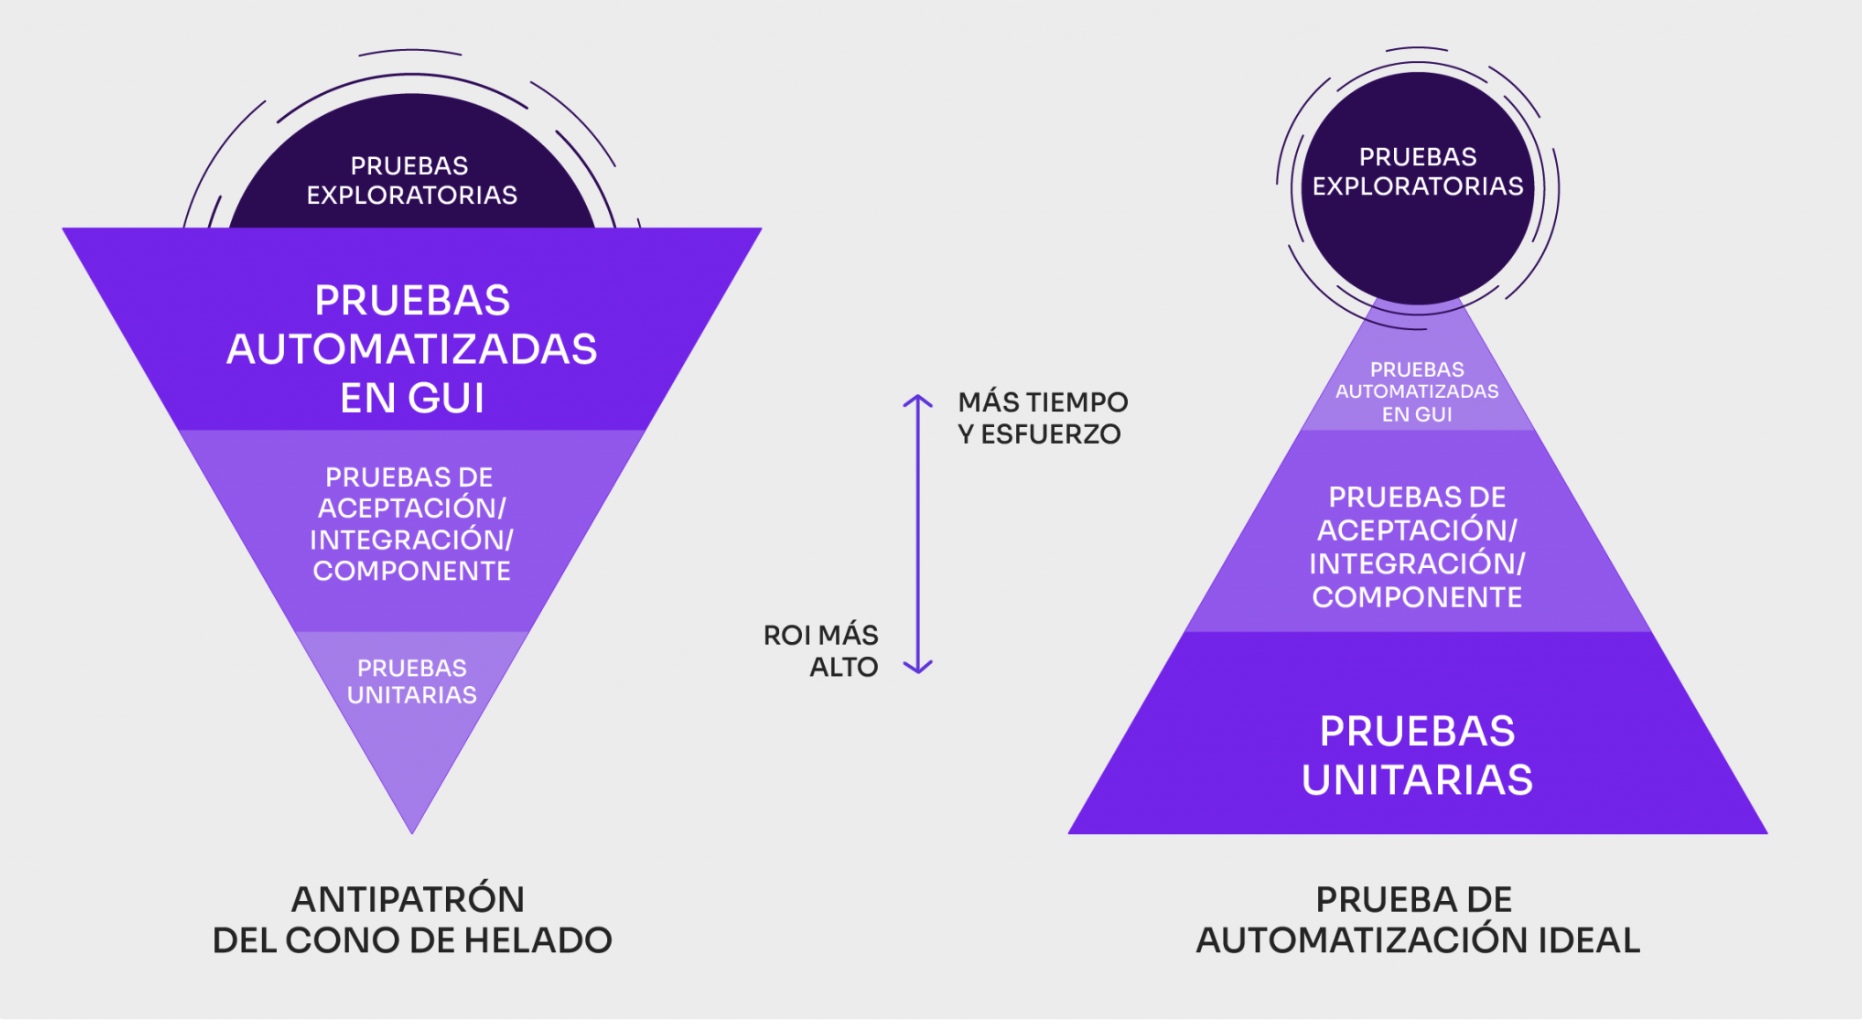
\includegraphics[height=0.35\textheight]{./part/Proyecto_ejecutivo/memoria_descriptiva/prestaciones/TestPiramid}
        \caption{Piramides de distribución de pruegbas: patrón y antipatrón}\label{fig:piramidTest}
    \end{figure}

\paragraph{Garantías de robustez ante nuevos desarrollo}
El fichero de definición de una imagen Docker se nombra por defecto como \textit{Dockerfile}.
Expresa la imagen base desde la que se parte, el fichero diseñado usa un sistema operativo debian, y se procede a ejecutar los distintos pasos de instalación de dependencias que se requieren para construir el contenedor.
En un mismo fichero Dockerfile existen distintos stages.
Un stage es cada conjunto de pasos diferenciados por un nombre.
A la hora de levantar el contenedor se puede seleccionar el requerido.
Esto es útil para, en un mismo fichero, especificar si queremos instalar las dependencias para desarrollo o producción.
Así se especifican y ahorran los elementos comunes, que de otro modo habrían de duplicarse y mantener en ficheros separados.
Los stages diseñados son: base, dev, compile y prod.

En la base se instalan los elementos comunes.
Si se especifica dev entonces se instala Golang, el debugger Delve, un usuario para evitar el uso de sudo dentro dicho container y distintas utilidades generales como git, vim como editor de textos y fish como terminal.
Si se construye mediante la etiqueta \textit{compile} se evita la instalación de los elementos de desarrollo y sólo instalamos golang para poder compilar el código.
En prod se usa esa fase primero para compilar.
Luego se parte de la base en limpio y se crea un contenedor con el ejecutable en su interior.
Ahorrando espacio en el contenedor.
Estos pasos pueden apreciarse en la~\cref{lst:dockerfile}.

La infraestructura consta además de una red para hacer visible los contenedores entre si: Manager, clients, base de datos y el proxy para el RPC\@.
La estructura se especifica en un archivo docker-compose.yml .~\cref{lst:dockercompose}.
Habrá un docker-compose.yml aparte para el proxy y la base de datos~\cref{lst:dockercomposegen}.

\phantom{blank}
\vspace{10mm}

\hrule

\begin{lstlisting}[language=docker-compose-2,caption={Docker-compose.yml para cada proyecto golang: Manager, client y control},breaklines=true,label={lst:dockercompose}]
version: "3.9"
services:
    web:
        container_name: go-manager
        build:
            context: .
            dockerfile: docker/Dockerfile
            target: $target
            args:
                GO_VERSION: 19.2
        image: go-manager:19.2-${target}
        ports:
            - "8081:8081"
            - "40000:40000"
        security_opt:
            - "seccomp:unconfined"
        cap_add:
            - SYS_PTRACE
        volumes:
            - .:/app
        tty: true

networks:
    default:
        name: pfm-network
        external: true
\end{lstlisting}


\hrule

\begin{lstlisting}[language=docker-compose-2,caption={Docker-compose.yml de sistemas compartidos y network},breaklines=true,label={lst:dockercomposegen}]
version: "3.9"

services:
  envoy:
    build:
      context: .
      dockerfile: ./envoy/Dockerfile
    image: grpcweb/envoy
    ports:
      - "8080:8080"
      - "9901:9901"
  mysql:
    image: mysql:8.0
    ports:
      - "127.0.0.1:3306:3306"
    container_name: mysql
    command: --default-authentication-plugin=mysql_native_password --general-log=1 --general-log-file=/tmp/mysql.log
    user: "1000:1000"
    environment:
      - MYSQL_ROOT_PASSWORD=$MYSQL_ROOT_PASSWORD
      - MYSQL_DATABASE=$MYSQL_DATABASE
    volumes:
      - pfm-db-data:/var/lib/mysql
volumes:
  pfm-db-data:
networks:
  default:
    name: pfm-network
    external: true
\end{lstlisting}


\hrule

\begin{lstlisting}[language=docker,caption={Dockerfile.yml},breaklines=true,label={lst:dockerfile}]
FROM debian:buster AS base

ARG GO_VERSION
RUN apt update && apt install -y curl

FROM base AS dev

WORKDIR /tmp

RUN apt update && apt install -y build-essential curl vim fish git sudo \
    && groupadd -g 1000 docker-user \
    && useradd -d /home/docker-user -s /bin/bash -u 1000 -g 1000 docker-user \
    && usermod -aG sudo docker-user && echo "docker-user:1234" | sudo chpasswd \
    && mkdir /home/docker-user \
    && chown -R docker-user:docker-user /home/docker-user

USER docker-user
WORKDIR /home/docker-user

RUN URL=https://storage.googleapis.com/golang/go1.${GO_VERSION}.linux-amd64.tar.gz \
        && curl ${URL} -o go.tar.gz  \
        && tar -zxf go.tar.gz  \
        && rm -rf go.tar.gz

ENV GOPATH /home/docker-user/go
ENV PATH $PATH:/home/docker-user/go/bin
ENV CGO_ENABLED 0

RUN go install github.com/go-delve/delve/cmd/dlv@latest
RUN ls -s /home/docker-user/go/bin/dlv /usr/local/bin

WORKDIR /app

FROM base AS compile

WORKDIR /tmp
RUN URL=https://storage.googleapis.com/golang/go1.${GO_VERSION}.linux-amd64.tar.gz \
        && curl ${URL} -o go.tar.gz  \
        && tar -zxf go.tar.gz  \
        && rm -rf go.tar.gz  \
        && mv go /usr/local/go

ENV GOPATH /usr/local/go
ENV PATH $PATH:/usr/local/go/bin
# If you enable this, then gcc is needed to debug your app
ENV CGO_ENABLED 0

WORKDIR /app
COPY ./app .
RUN go build -ldflags "-s -w" -o final.sh

FROM debian:buster AS prod

WORKDIR /
COPY --from=compile /app/final.sh /
CMD ["./final.sh"]
\end{lstlisting}

\hrule





